Di seguito verranno presentati i diagrammi di attività che descrivono le iterazioni tra l'utente e il software \PROGETTO.
\'E stato disegnato un diagramma ad alto livello che descrive le attività principali, le quali verranno poi analizzate in dettaglio tramite dei sotto-diagrammi specifici. Per rendere la lettura del diagramma più semplice, é stato scelto di usare il nome in rosso per le attività che sono da considerarsi di alto livello, descritte poi più approfonditamente in sotto-attività tramite i relativi diagrammi. I riquadri con testo normale invece sono invece da intendersi come singole attività.

\subsection{Attività principali}
L'utente una volta avviato il programma ha la possibilità di \textit{Effettuare una ricerca}, \textit{Visualizzare un progetto}, \textit{Registrarsi}, \textit{Autenticarsi} e, una volta autenticato, di \textit{Creare un nuovo progetto}, \textit{Aprire un progetto}, \textit{Modificare un progetto} e \textit{Salvare un progetto}. Queste sono le principali attività dell'applicazione e possono essere utilizzate in parallelo senza che le singole attività vengano interrotte (figura 2).

\begin{figure}[p] 
	\centering 
	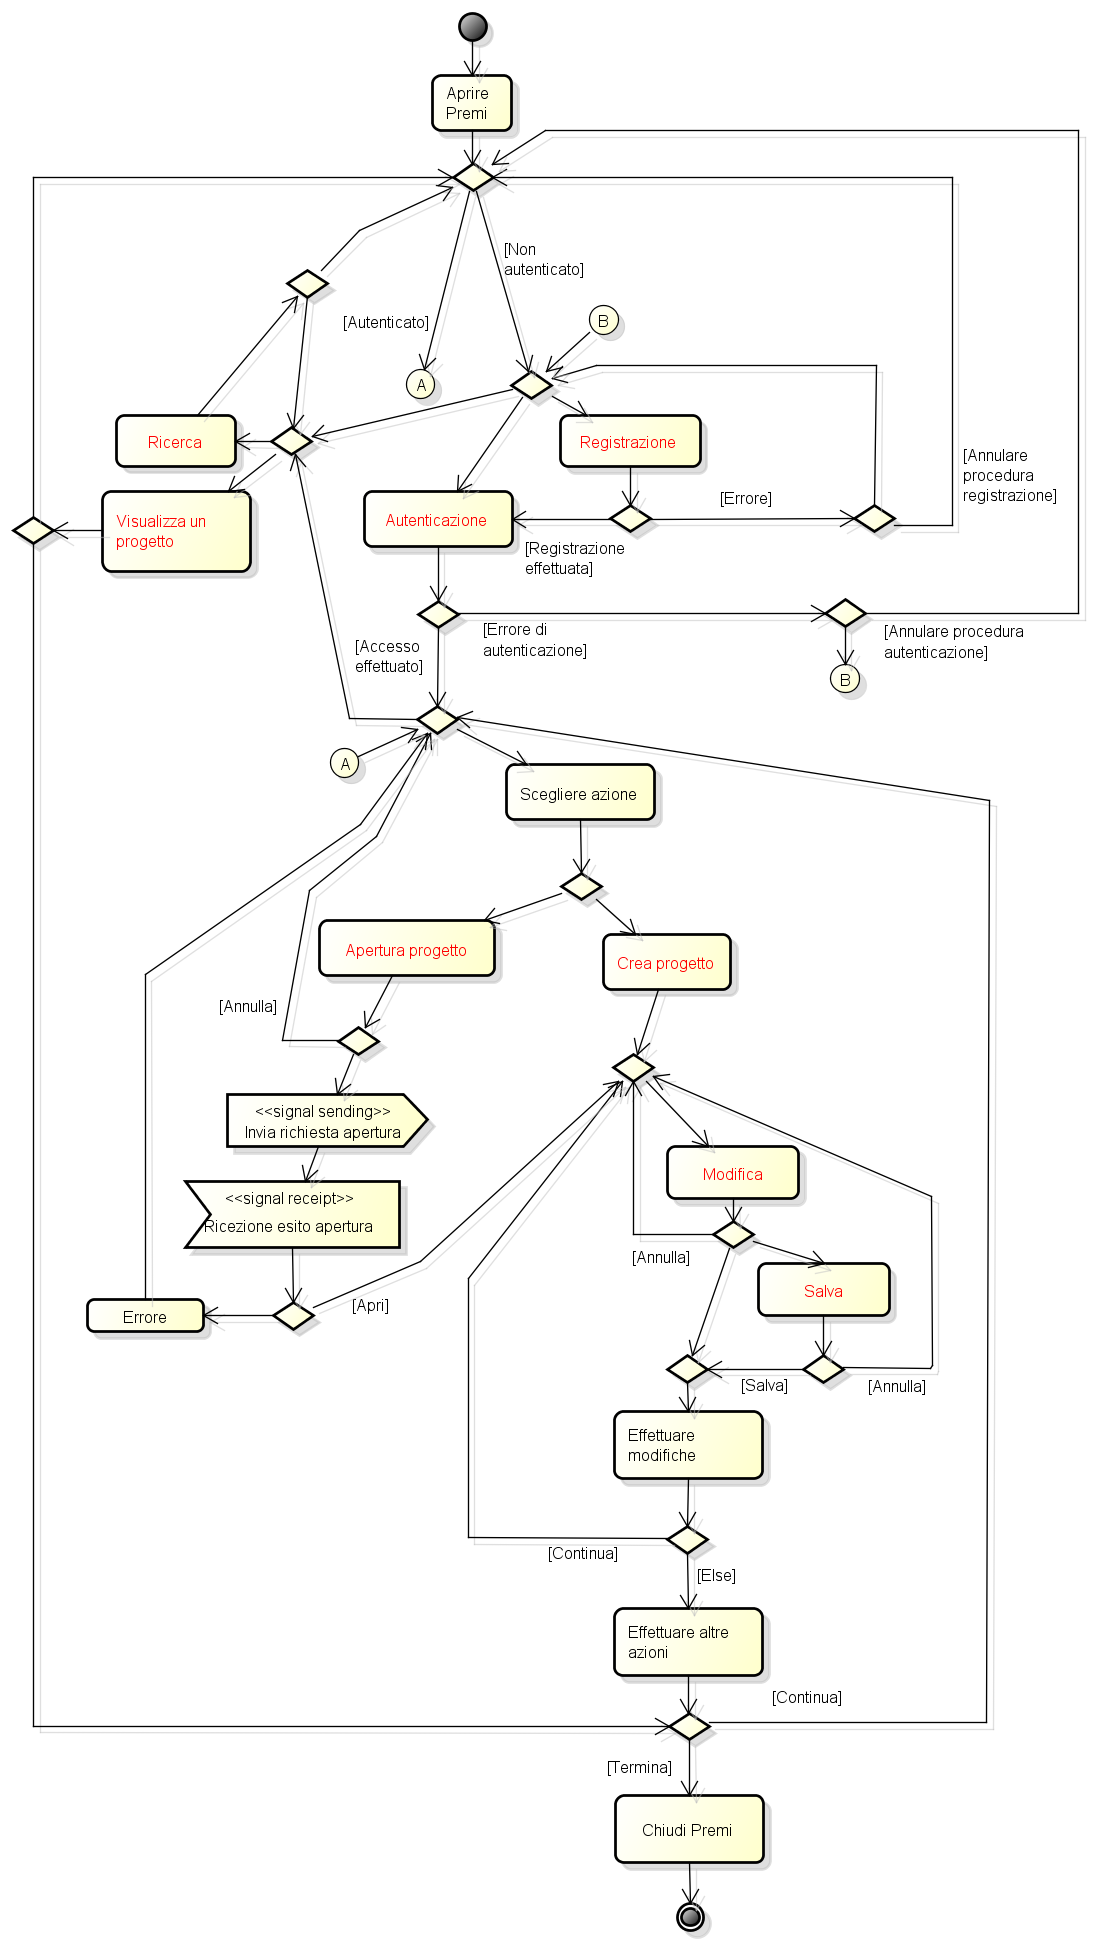
\includegraphics[height=20cm, keepaspectratio] {img/Activity_diagram.png} 
	\caption{Diagramma attività - Attività principali dell'applicativo \PROGETTO} 
\end{figure}

\newpage

\subsection{Ricerca di un progetto}
\begin{figure}[h] 
	\centering 
	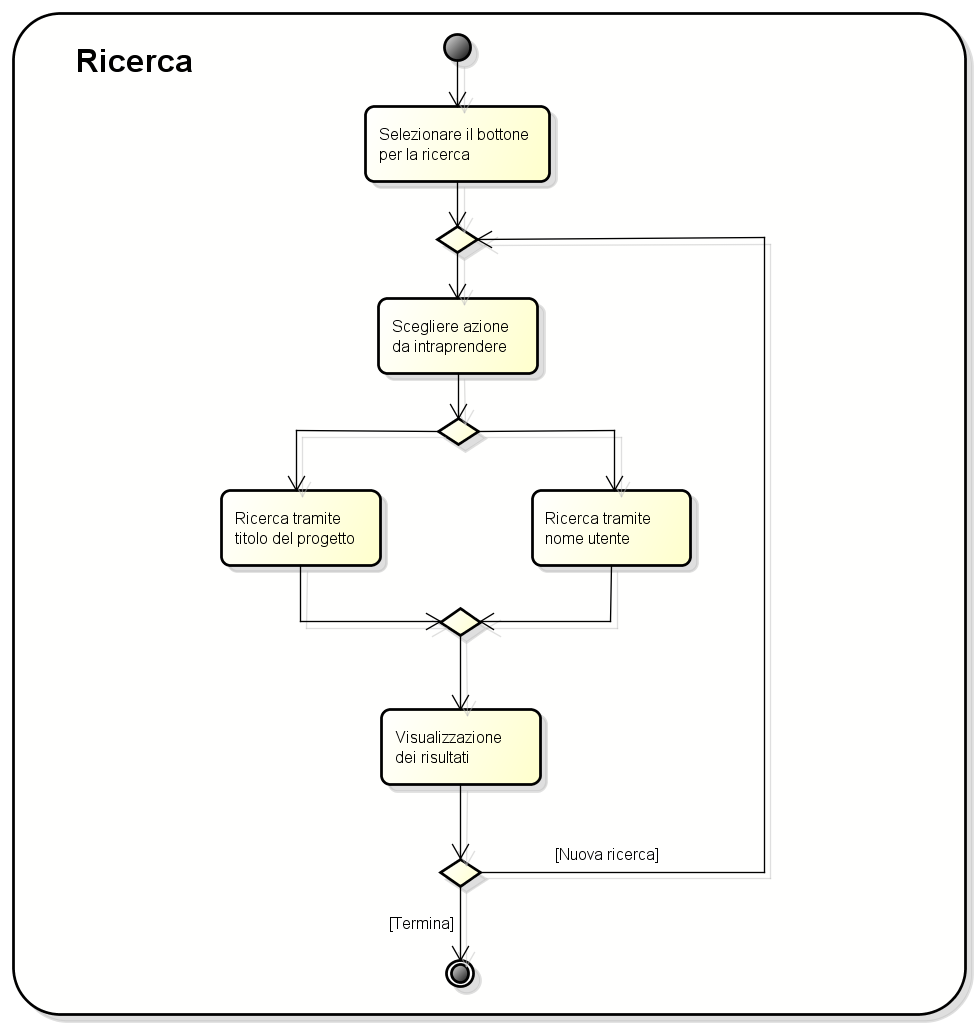
\includegraphics[scale=0.3] {img/Activity_ricerca.png} 
	\caption{Diagramma attività - Ricerca di un progetto} 
\end{figure}
L'attività di ricerca di un progetto in figura 3 comprende le azioni di ricerca tramite titolo del progetto, ricerca tramite nome utente e visualizzazione dei risultati della ricerca. Una volta visualizzati i risultati, opzionalmente l'utente può effettuare un'altra ricerca.
\newpage

\subsection{Visualizzare un progetto}
\begin{figure}[h] 
	\centering 
	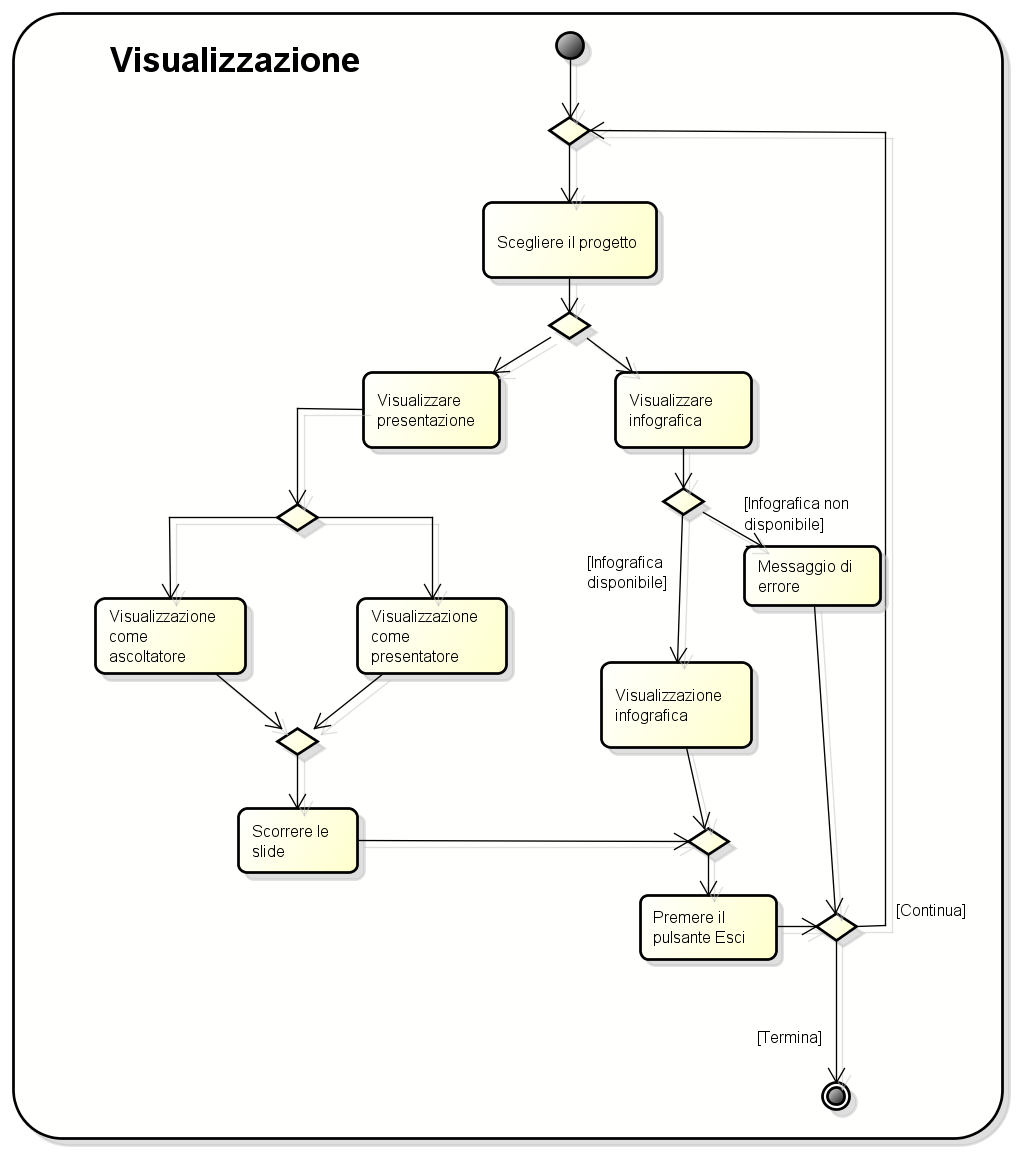
\includegraphics[scale=0.3] {img/Activity_visualizza.png} 
	\caption{Diagramma attività - Visualizzare un progetto} 
\end{figure}
L'attività di visualizzazione di un progetto in figura 4 permette all'utente, una volta scelto il progetto, di visualizzare la presentazione oppure l'\gls{infografica} legata al progetto (se essa é disponibile). Nel caso si scelga di visualizzare una presentazione l'utente può scegliere se visualizzarla in modalità ascoltatore o presentatore, una volta fatta la decisione si può muovere tra le slide.
\newpage


\subsection{Registrazione}
\begin{figure}[h] 
	\centering 
	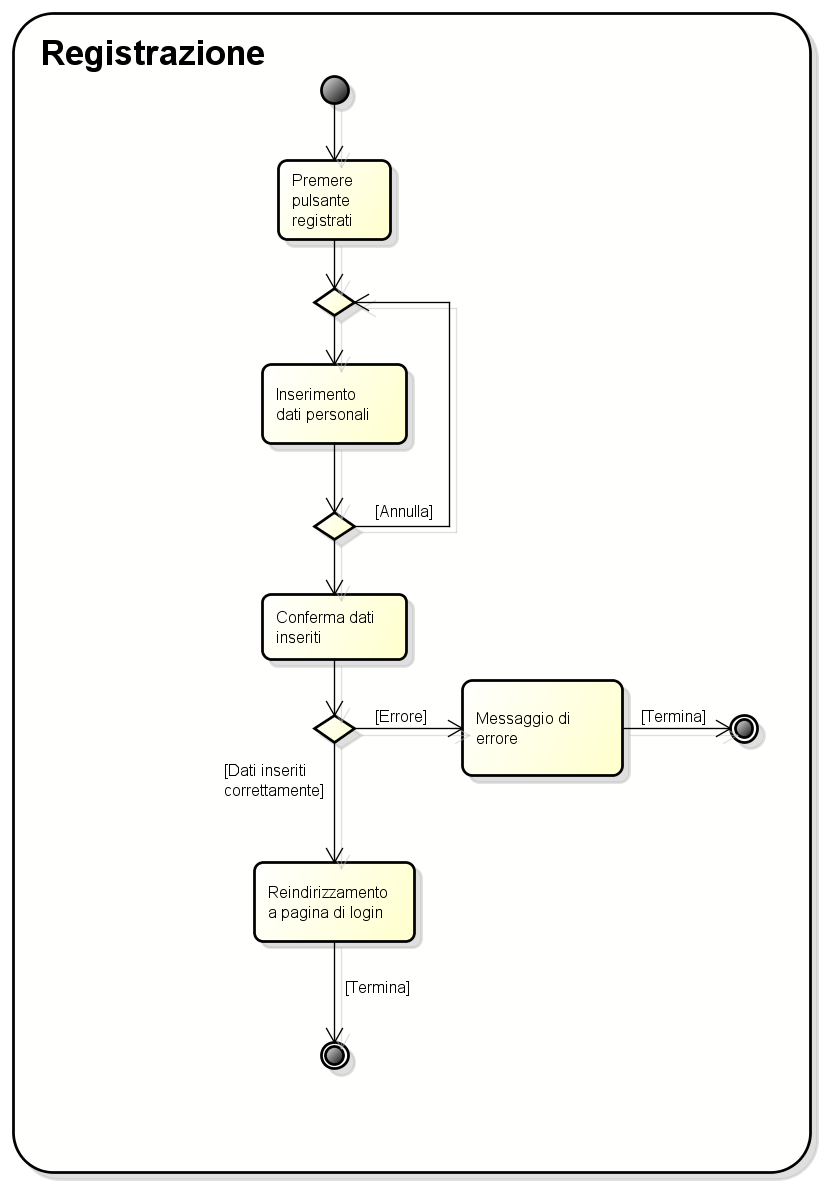
\includegraphics[scale=0.3] {img/Activity_registrazione.png} 
	\caption{Diagramma attività - Registrazione} 
\end{figure}
La figura 5 rappresenta l'attività di registrazione di un utente. Una volta premuto il pulsante di registrazione, l'utente deve inserire i propri dati e può scegliere di annullare l'inserimento di un dato e reinserirlo senza dover ripetere la procedura. Una volta confermati i dati inseriti, se corretti l'utente viene registrato e reindirizzato alla pagina di login.
\newpage


\subsection{Autenticazione}
\begin{figure}[h] 
	\centering 
	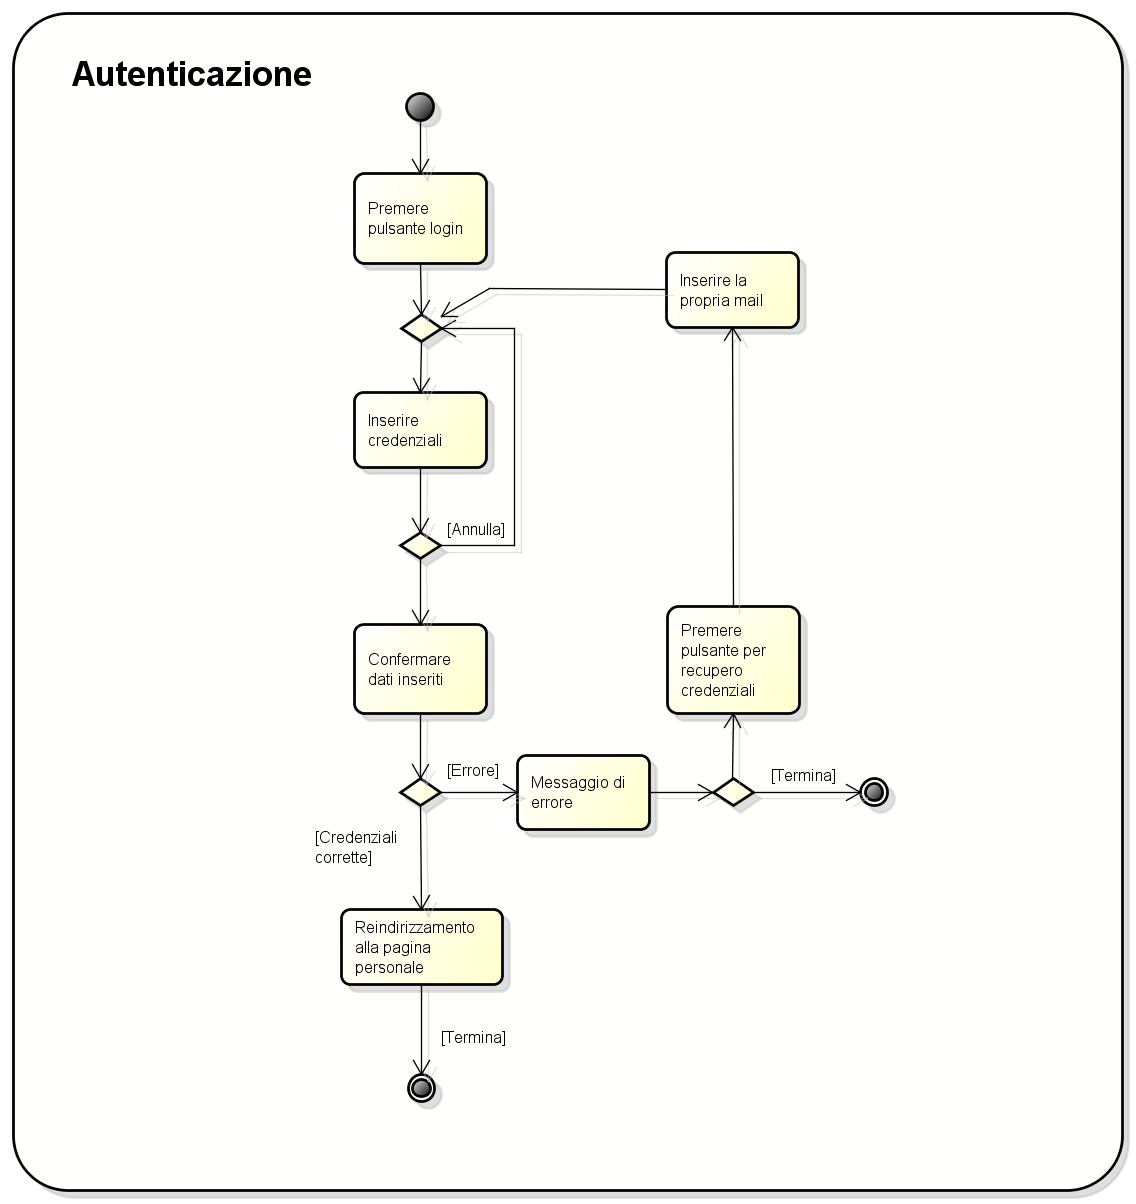
\includegraphics[scale=0.3] {img/Activity_autenticazione.png} 
	\caption{Diagramma attività - Autenticazione} 
\end{figure}
L'attività di autenticazione in figura 6 permette all'utente di inserire le proprie credenziali, di annullarne l'inserimento nel caso in cui si sbagli a digitarle e di confermarle. Nel caso in cui l'utente non ricordi più le proprie credenziali ha la possibilità di eseguire la procedura di recupero dei propri dati, alla fine della quale viene riportato alla pagina di login.
\newpage


\subsection{Creazione di un progetto}
\begin{figure}[h] 
	\centering 
	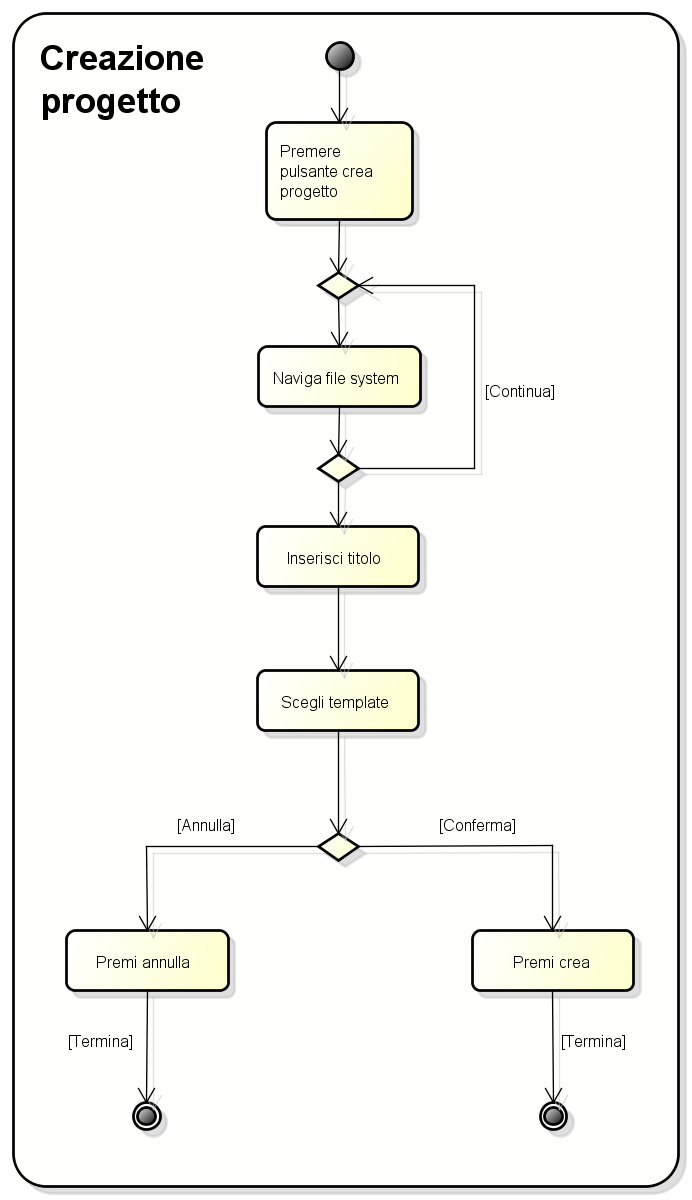
\includegraphics[scale=0.3] {img/Activity_creazione.png} 
	\caption{Diagramma attività - Creazione di un progetto} 
\end{figure}
L'attività di creazione in figura 7 permette ad un utente autenticato di creare un nuovo progetto, di selezionare dove sarà salvato il progetto e richiede di inserire un titolo e di scegliere un template.
\newpage


\subsection{Apertura di un progetto}
\begin{figure}[h] 
	\centering 
	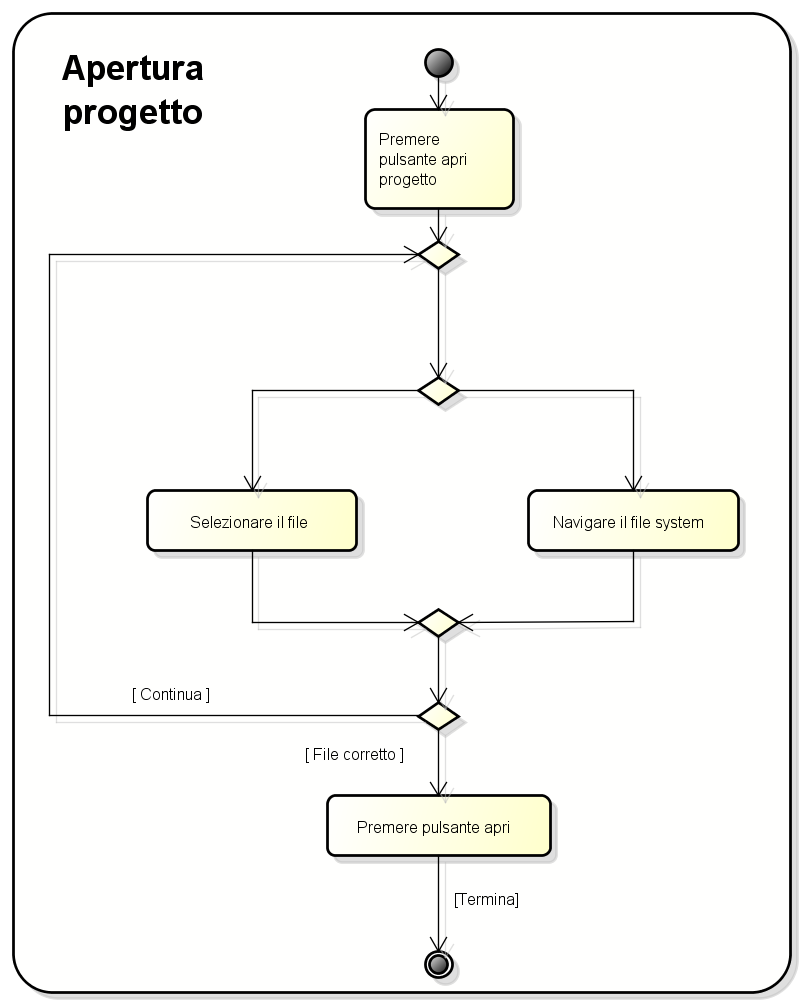
\includegraphics[scale=0.3] {img/Activity_apertura.png} 
	\caption{Diagramma attività - Apertura di un progetto} 
\end{figure}
L'attività di apertura di un progetto in figura 8 permette all'utente di navigare il file system e di scegliere quale progetto deve essere aperto.
\newpage

\subsection{Modifica di un progetto}
\begin{figure}[h] 
	\centering 
	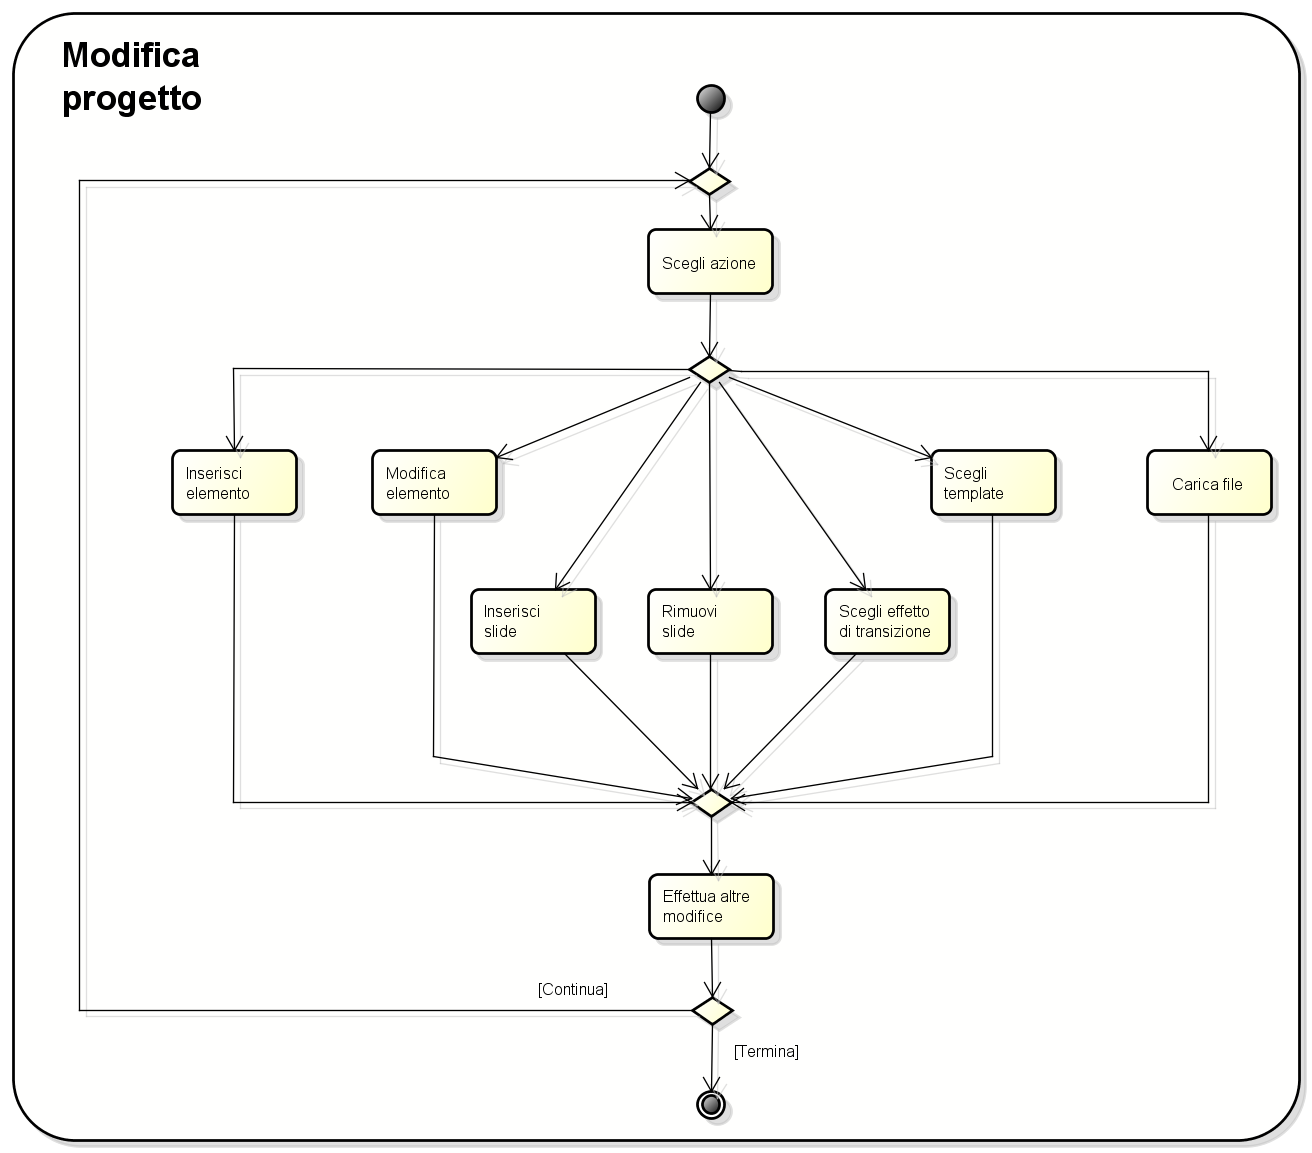
\includegraphics[scale=0.3] {img/Activity_modifica.png} 
	\caption{Diagramma attività - Modifica di un progetto} 
\end{figure}
L'attività di modifica in figura 9 permette all'utente di inserire e modificare elementi (come testo, immagini, grafici, ecc...) nella presentazione corrente. L'utente può inoltre aggiungere e rimuovere slide, scegliere un diverso template e cambiare l'effetto di transizione tra una slide e l'altra.
\newpage

\subsection{Salvataggio di un progetto}
\begin{figure}[h] 
	\centering 
	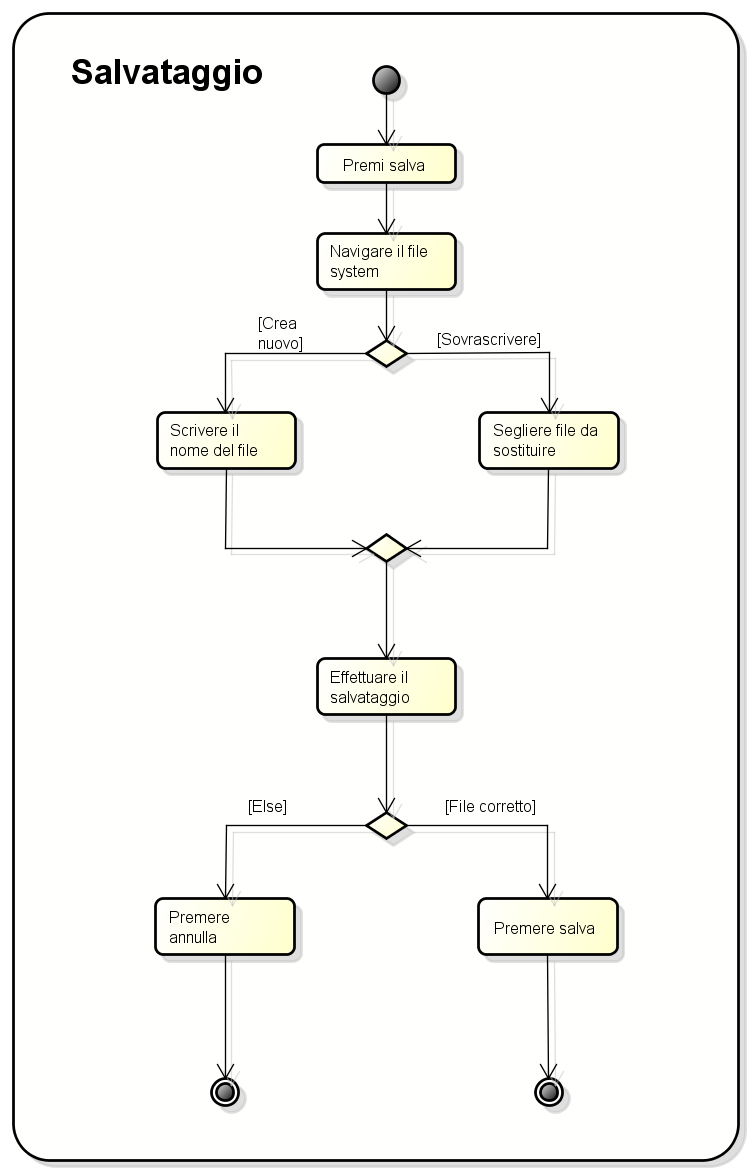
\includegraphics[scale=0.3] {img/Activity_salvataggio.png} 
	\caption{Diagramma attività - Salvataggio di un progetto} 
\end{figure}
La figura 10 rappresenta l'attività di salvataggio di un progetto. Lo schema indica la possibilità per l'utente di navigare il file system e di scegliere un nome per il progetto da salvare o di selezionare un progetto già esistente da sovrascrivere.
\newpage